\documentclass[12pt, titlepage]{article}

\usepackage{amsmath, mathtools}

\usepackage[round]{natbib}
\usepackage{amsfonts}
\usepackage{amssymb}
\usepackage{graphicx}
\usepackage{colortbl}
\usepackage{xr}
\usepackage{hyperref}
\usepackage{longtable}
\usepackage{xfrac}
\usepackage{tabularx}
\usepackage{float}
\usepackage{siunitx}
\usepackage{booktabs}
\usepackage{multirow}
\usepackage[section]{placeins}
\usepackage{caption}
\usepackage{fullpage}
\externaldocument{../../SRS/SRS} 
\externaldocument{../MG/MG}
\hypersetup{
bookmarks=true,     % show bookmarks bar?
colorlinks=true,       % false: boxed links; true: colored links
linkcolor=red,          % color of internal links (change box color with linkbordercolor)
citecolor=blue,      % color of links to bibliography
filecolor=magenta,  % color of file links
urlcolor=cyan          % color of external links
}

\usepackage{array}
\newcommand{\rref}[1]{R\ref{#1}}
\newcommand{\ddref}[1]{DD\ref{#1}}
\newcommand{\mref}[1]{M\ref{#1}}
%% Comments

\usepackage{color}

\newif\ifcomments\commentstrue

\ifcomments
\newcommand{\authornote}[3]{\textcolor{#1}{[#3 ---#2]}}
\newcommand{\todo}[1]{\textcolor{red}{[TODO: #1]}}
\else
\newcommand{\authornote}[3]{}
\newcommand{\todo}[1]{}
\fi

\newcommand{\wss}[1]{\authornote{blue}{SS}{#1}}
\newcommand{\an}[1]{\authornote{magenta}{Author}{#1}}


\newcommand{\progname}{Program Name}

\begin{document}

\title{Module Interface Specification for ...}

\author{Author Name}

\date{\today}

\maketitle

\pagenumbering{roman}

\section{Revision History}

\begin{tabularx}{\textwidth}{p{3cm}p{2cm}X}
\toprule {\bf Date} & {\bf Version} & {\bf Notes}\\
\midrule
Date 1 & 1.0 & Notes\\
Date 2 & 1.1 & Notes\\
\bottomrule
\end{tabularx}

~\newpage

\section{Symbols, Abbreviations and Acronyms}

See SRS Documentation at \wss{give url}

\wss{Also add any additional symbols, abbreviations or acronyms}

\newpage

\tableofcontents

\newpage

\pagenumbering{arabic}

\section{Introduction}

The following document details the Module Interface Specifications for Breaking Effect.
 
Breaking effect presents how the pieces of an object move after it separates into parts with
suddenness or violence.

This project implements running time breaking effect in codes for 3-D models in unity3D without help from any similar plug-in. Including different shapes 3-D objects breaking based on physics and pieces interacting with the momentum provided by the breaking force. The breaking effect program simulates 3-D objects destruction process in vision by implementing scientific computing functions.

This project concentrates on calculation while
HCI or GUI are not important parts. Applied force is decided in codes in advance as input
and trace of motion is the output after calculation.

Complementary documents include the System Requirement Specifications
and Module Guide.  The full documentation and implementation can be
found at \url{https://github.com/MaXiaoye/cas741}.

\section{Notation}

\wss{You should describe your notation.  You can use what is below as
  a starting point.}

The structure of the MIS for modules comes from \citet{HoffmanAndStrooper1995},
with the addition that template modules have been adapted from
\cite{GhezziEtAl2003}.  The mathematical notation comes from Chapter 3 of
\citet{HoffmanAndStrooper1995}.  For instance, the symbol := is used for a
multiple assignment statement and conditional rules follow the form $(c_1
\Rightarrow r_1 | c_2 \Rightarrow r_2 | ... | c_n \Rightarrow r_n )$.

The following table summarizes the primitive data types used by \progname. 

\begin{center}
\renewcommand{\arraystretch}{1.2}
\noindent 
\begin{tabular}{l l p{7.5cm}} 
\toprule 
\textbf{Data Type} & \textbf{Notation} & \textbf{Description}\\ 
\midrule
character & char & a single symbol or digit\\
integer & $\mathbb{Z}$ & a number without a fractional component in (-$\infty$, $\infty$) \\
natural number & $\mathbb{N}$ & a number without a fractional component in [1, $\infty$) \\
real & $\mathbb{R}$ & any number in (-$\infty$, $\infty$)\\
\bottomrule
\end{tabular} 
\end{center}

\noindent
The specification of \progname \ uses some derived data types: sequences, strings, and
tuples. Sequences are lists filled with elements of the same data type. Strings
are sequences of characters. Tuples contain a list of values, potentially of
different types. In addition, \progname \ uses functions, which
are defined by the data types of their inputs and outputs. Local functions are
described by giving their type signature followed by their specification.

\section{Module Decomposition}

The following table is taken directly from the Module Guide document for this project.

\begin{table}[h!]
	\centering
	\begin{tabular}{p{0.3\textwidth} p{0.6\textwidth}}
		\toprule
		\textbf{Level 1} & \textbf{Level 2}\\
		\midrule
		
		{Hardware-Hiding Module} & ~ \\
		\midrule
		
		\multirow{7}{0.3\textwidth}{Behaviour-Hiding Module} & Input Module\\
		& Obtaining gravity center module\\
		& Angle calculation module\\
		& Displacement in the air calculation module\\
		& Displacement on the ground calculation module\\
		\midrule
		
		\multirow{3}{0.3\textwidth}{Software Decision Module} & Object cutting module\\
		& Output Module\\
		\bottomrule
		
	\end{tabular}
	\caption{Module Hierarchy}
	\label{TblMH}
\end{table}

\begin{figure}[H]
	\centering
	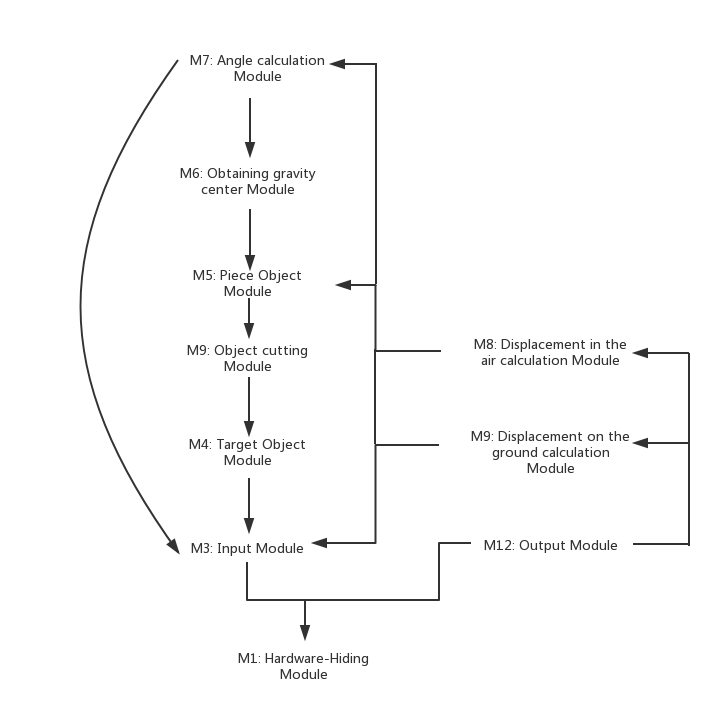
\includegraphics[width=0.7\textwidth]{./Figure1.png}
	\caption{Use hierarchy among modules}
	\label{FigUH}
\end{figure}

\newpage
~\newpage

\section{MIS of Input Module(\mref{mIF})} 

This module collect input data to do verification and store in corresponding variables. Include position of target object, explosion level, coefficient of ground friction. \an{Time is input provided by Unity3D.}\\
\an{Can I put description here?}

\subsection{Module}

InputModule

\subsection{Uses}

Hardware-Hiding Module (\mref{mHH})

\subsection{Syntax}



\subsubsection{Exported Access Programs}

\begin{center}
\begin{tabular}{p{2cm} p{4cm} p{4cm} p{2cm}}
\hline
\textbf{Name} & \textbf{In} & \textbf{Out} & \textbf{Exceptions} \\
\hline
GetInitPos & TargetObject & $\mathbb{R}$ & InvalidObject \\
InputVerifiy & $\mathbb{R}$ & void & OutOfScope \\
\hline
\end{tabular}
\end{center}

\subsection{Semantics}

\subsubsection{State Variables}
\an{Input module may not have state variables. But it do return different result depends on input data ?}
\subsubsection{Access Routine Semantics}

\noindent GetInitPos():
\begin{itemize}
	\item transition: \an{No transition}
	\item output: $X = Object.X; Y = Object.Y; Z = Object.Z$. $(X,Y,Z):\mathbb{R}$ \an{No output but assignment}
	\item exception: exc := (TargetObject = null $\Rightarrow $ NoObjectException)
\end{itemize}

\noindent InputVerifiy():
\begin{itemize}
\item transition: N/A
\item output: Exceptions or None.
\item exception:\an{Different kinds of exceptions for different invalid inputs.}\\
exc := ($\mu_{k}$ = null $\Rightarrow $ NoMuException)\\
exc := (ExplosionLv = null $\Rightarrow $ NoELvException)\\
exc := ($X,Y,Z \notin \mathbb{R} \vee (X,Y,Z \le -1000) \vee (X,Y,Z \ge 1000)$ $\Rightarrow $ InvalidCoorException)\\
exc := ($E \notin \mathbb{R} \vee (E \leq 0) \vee (E \geq 10)$ $\Rightarrow $ InvalidELvException)\\
exc := ($\mu_{k} \notin \mathbb{R} \vee (\mu_{k} \le 0) \vee (\mu_{k} \ge 1)$ $\Rightarrow $ InvalidMuException)\\
\end{itemize}

\section{MIS of Obtaining gravity center module (\mref{mOGC})} 

Call cutting function provided by Unity3D to split target object into pieces then do traversal to obtain gravity centers of all pieces. \an{Each piece is an object. Gravity center is a value in PieceObj}

\subsection{Module}

ObtainGCModule

\subsection{Uses}

Input Module(\mref{mIF})\\
Object cutting module(\mref{mOC})\\

\subsection{Syntax}

\subsubsection{Exported Access Programs}

\begin{center}
	\begin{tabular}{p{2cm} p{4cm} p{4cm} p{2cm}}
		\hline
		\textbf{Name} & \textbf{In} & \textbf{Out} & \textbf{Exceptions} \\
		\hline
		CuttingFun & TargetObject & PieceObj & ExternalException \\
		Traverse & PieceObj;$\mathbb{R}$ & List of PieceObj & -\\
		\hline
		
	\end{tabular}
\end{center}
\an{Put all functions in the table or in Access Routine Semantics part?}

\subsection{Semantics}

\subsubsection{State Variables}
\an{No state variables}
\subsubsection{Access Routine Semantics}

\an{Do I need to put variables here?}

\noindent Traverse():
\begin{itemize}
	\item transition: PieceObj $\rightarrow$ List of PieceObj \an{data type change?}
	\item output: List of PieceObj 
	\item exception: None
\end{itemize}

\section{MIS of Angle calculation module(\mref{mAC})} 
Calculate the angle between initial speed $v_{0}$ and horizontal $\theta_{1}$. Calculate the angle between $x$ axiom and projection on horizontal of initial speed $\theta_{2}$. \an{$\theta_{1}$ and $\theta_{2}$ are values of each PieceObj}\\
\an{Can I put equations in IM here?}\\
$\theta_{1}=arctan \frac{|z_{n}|}{\sqrt{(x_{n}-X)^2+(y_{n}-Y)^2}}$\\
$\theta_{2}=arctan \frac{|y_{n}-Y|}{|x_{n}-X|}$
\subsection{Module}

AngleCalModule

\subsection{Uses}

Input Module(\mref{mIF})\\
Obtaining gravity center module (\mref{mOGC})

\subsection{Syntax}

\subsubsection{Exported Access Programs}

\begin{center}
	\begin{tabular}{p{2cm} p{4cm} p{4cm} p{2cm}}
		\hline
		\textbf{Name} & \textbf{In} & \textbf{Out} & \textbf{Exceptions} \\
		\hline
		AngleSH & $\mathbb{R}$;PieceObj & $\mathbb{R}$ & - \\
		AngleXV & $\mathbb{R}$;PieceObj & $\mathbb{R}$ & - \\
		\hline
	\end{tabular}
\end{center}

\subsection{Semantics}

\subsubsection{State Variables}

None

\subsubsection{Access Routine Semantics}

\noindent AngleSH():
\begin{itemize}
	\item transition: \an{No transition}   
	\item output: $\theta_{1}: \mathbb{R}$
	\item exception: None
\end{itemize}

\noindent AngleXV():
\begin{itemize}
	\item transition: \an{No transition}  
	\item output: $\theta_{2}: \mathbb{R}$
	\item exception: None
\end{itemize}

\section{MIS of Displacement in the air calculation module(\mref{mDC1})}

Calculate and output trace of motion for each piece in the air by using follow equations.\\
$S_{x}=v_{0}\cdot cos\theta _{1}\cdot cos\theta _{2}\cdot t$\\
$S_{y}=v_{0}\cdot cos\theta _{1}\cdot sin\theta _{2}\cdot t$,\\
$S_{z}=v_{0}\cdot sin\theta _{1}\cdot t-\frac{1}{2}gt^{2}$
\an{S is displacement in one frame, t is the gap between each frame($\delta t$).}
\subsection{Module}

DisAirCalModule

\subsection{Uses}

Input Module(\mref{mIF})\\
Angle calculation module(\mref{mAC})\\

\subsection{Syntax}

\subsubsection{Exported Access Programs}

\begin{center}
	\begin{tabular}{p{2cm} p{4cm} p{4cm} p{2cm}}
		\hline
		\textbf{Name} & \textbf{In} & \textbf{Out} & \textbf{Exceptions} \\
		\hline
		DisAirCal & $\mathbb{R}$; PieceObj; TargetObject & $\mathbb{R}$ & - \\
		\hline
	\end{tabular}
\end{center}

\subsection{Semantics}

\subsubsection{State Variables}

onGround: Boolean \an{It is a variable in each PieceObj. That means program checks this variable each frame to call different IM as well as using equations}

\subsubsection{Access Routine Semantics}

\noindent DisAirCal():
\begin{itemize}
	\item transition: None
	\item output: $S_{x},S_{y},S_{z}: \mathbb{R}$ 
	\item exception: None
\end{itemize}

\section{MIS of Displacement on the ground calculation module(\mref{mDC2})}
Calculate and output trace of motion for each piece on the ground by using follow equations.\\
$S_{x}=v_{0}\cdot cos\theta _{1}\cdot cos\theta _{2}\cdot t-\frac{1}{2}at^{2}$\\
$S_{y}=v_{0}\cdot cos\theta _{1}\cdot sin\theta _{2}\cdot t-\frac{1}{2}at^{2}$
\subsection{Module}

DisGroCalModule

\subsection{Uses}

Input Module(\mref{mIF})
Angle calculation module(\mref{mAC})

\subsection{Syntax}

\subsubsection{Exported Access Programs}

\begin{center}
	\begin{tabular}{p{2cm} p{4cm} p{4cm} p{2cm}}
		\hline
		\textbf{Name} & \textbf{In} & \textbf{Out} & \textbf{Exceptions} \\
		\hline
		DisGroCal & $\mathbb{R}$; PieceObj; TargetObject & $\mathbb{R}$ & - \\
		\hline
	\end{tabular}
\end{center}

\subsection{Semantics}

\subsubsection{State Variables}

onGround: Boolean

\subsubsection{Access Routine Semantics}

\noindent DisGroCal():
\begin{itemize}
	\item transition: $a=\mu_{k}g$ \an{$a$ is intermediate result.}
	\item output: $S_{x},S_{y},S_{z}: \mathbb{R}$ 
	\item exception: None 
\end{itemize}

\section{MIS of Object cutting Module(\mref{mOC})} \label{mOC}

External function provided by platform

\subsection{Module}

ObjCutModule

\subsection{Uses}

Input Module(\mref{mIF})

\subsection{Syntax}

\subsubsection{Exported Access Programs}

\begin{center}
	\begin{tabular}{p{2cm} p{4cm} p{4cm} p{2cm}}
		\hline
		\textbf{Name} & \textbf{In} & \textbf{Out} & \textbf{Exceptions} \\
		\hline
		cut() & TargetObj & PieceObj & - \\
		\hline
	\end{tabular}
\end{center}

\subsection{Semantics}

\subsubsection{State Variables}

None

\subsubsection{Access Routine Semantics}

\noindent cut():
\begin{itemize}
	\item transition:  TargetObj $\rightarrow$ PieceObj
	\item output: PieceObj 
	\item exception: None 
\end{itemize}

\section{MIS of Output Module(\mref{mOM})}

\an{Unity3D interface with codes by calling function update() each frame. Unity3D convert data into visualization.}

\subsection{Module}

Output Module

\subsection{Uses}

Displacement in the air calculation module(\mref{mDC1})\\
Displacement on the ground calculation module(\mref{mDC2})\\

\subsection{Syntax}

\subsubsection{Exported Access Programs}

\begin{center}
	\begin{tabular}{p{2cm} p{4cm} p{4cm} p{2cm}}
		\hline
		\textbf{Name} & \textbf{In} & \textbf{Out} & \textbf{Exceptions} \\
		\hline
		update() & - & Visualization & - \\
		traverseDis() & List of PieceObj & - & - \\
		translate() & $\mathbb{R}$ & Visualization & - \\
		\hline
	\end{tabular}
\end{center}
\an{Call translate() function for all PieceObj each frame}
\subsection{Semantics}

\subsubsection{State Variables}

\subsubsection{Access Routine Semantics}

\noindent update():
\begin{itemize}
	\item transition: $\mathbb{R} \rightarrow$ Visualization 
	\item output: None 
	\item exception: None  
\end{itemize}

\newpage

\bibliographystyle {plainnat}
\bibliography {../../../ReferenceMaterial/References}

\newpage

\section{Appendix} \label{Appendix}

\wss{Extra information if required}

\end{document}
